\chapter{Expansion of the Parameter Space}
\label{chap: A_s}

Now that we have a comprehensive set of convenience functions with which to
configure CAMB, we can easily obtain the theoretical power spectra we need in
order to demonstrate our solution to the neutrino difficulties introduced in
section~\ref{sec: neutrino_problem}. This chapter will motivate the inclusion 
of the additional parameter $A_s$ in the evolution mapping framework.
Because the focus of this thesis is regression rather than theory,
we will merely show that $A_s$ contains information relevant to the impact of
massive neutrinos. Then, the GPR should, in principle, be able to optimize its
use to predict power spectra.

% Maybe it would make more sense to have the large cass-L chapter focus on the
% creation of a massless-neutrino emulator and THEN a smaller chapter focusing
% on all the changes necessary for it to become a massive-neutrino emulator.
% BUT! As of 25-08-23, I'm running way behind on writing actual content for
% this thesis. I can't risk redoing all the section headers again. We're
% going to proceed under the current scheme and MAYBE allow ourselves to redo
% it shortly before submission.

\section{Equation to be Solved}

% Redo section title

\textcolor{orange}{Remember to explain \textit{why} the prediction of these 
asymptotes means that $A_s$ will capture most of the unruly behavior of 
neutrinos. What theory motivates such a judgment? Or are we only guessing?}

We begin with the second proposal from section~\ref{sec: neutrino_problem}:
to approximate the power spectrum of a massive-neutrino cosmology, we
combine the
power spectrum of its MEMNeC with an approximation of the ratio
between the two:

\begin{equation}
\label{eq: MEMNeC_approx}
P_\nu(k) \approx \de^* (k) P_0 (k)
,\end{equation}

The essence of this chapter is to increase the accuracy in our $P_\nu(k)$
predictions by estimating the true $\de(k)$. Specifically, we are interested
in how the true $\de(k)$ deviates from $\de^*(k)$. Therefore, we pay special
attention to the quantity:

\begin{equation}
\label{eq: ee}
\ee (k) \equiv \frac{\de(k)}{\de^*(k)}
\end{equation}

To simplify the discussion, we will concentrate on the small-scale limit of 
this ratio $\el$

\begin{equation}
\el \equiv \lim_{k \rightarrow \infty} \ee(k)
\end{equation}

If we can estimate $\el$ accurately, then in principle our task 
is complete, because the slope toward smaller $k$ values is
even and analytically predictable. \textcolor{green}{Can I refer the reader to
 a paper on this?}

\section{Proposed Fitting Functions}
 
In order to explore this limit concretely, we will use the Aletheia models as
our test cases. This means that we can rewrite definition~\ref{eq: ee} as:

\begin{equation}
\label{eq: eei}
\ee_i (k) \equiv \frac{\de_\text{model i}(k)}{\de_\text{model 0}(k)}
\end{equation}

\textcolor{orange}{This section, like the ``Convenience Functions'' section
from chapter 2, should anticipate CL: we should talk about the
code that we have written in order to explore these ratios, which one can find
in} \verb|camb_interface.py|.

To study the behavior of $\ee_i$, we developed the \verb|camb_interface.py|
function \verb|model_ratios|. This function accepts a single snap
index\footnote{Remember that there are four snaps for each model, and snap 
four always corresponds to $z = 0$} and a set of power spectra nearly in the
format returned by \\
\verb|boltzmann_battery|, but without the $\omega_\nu$ 
layer.\footnote{For explanations of the
remaining function parameters, we refer the reader to the docstring} Tt
computes and plots all of the $\ee_i$ spectra in the input set. We show an
example output in figure~\ref{fig: model_ratios_demo}. This function
is recommended for any users seeking to improve the characterization of
$\ee_i$.

% The following plots were generated with divergence_asymptotes.ipynb
\begin{figure}[ht!]
    \begin{subfigure}{0.45 \textwidth}
    \centering
 		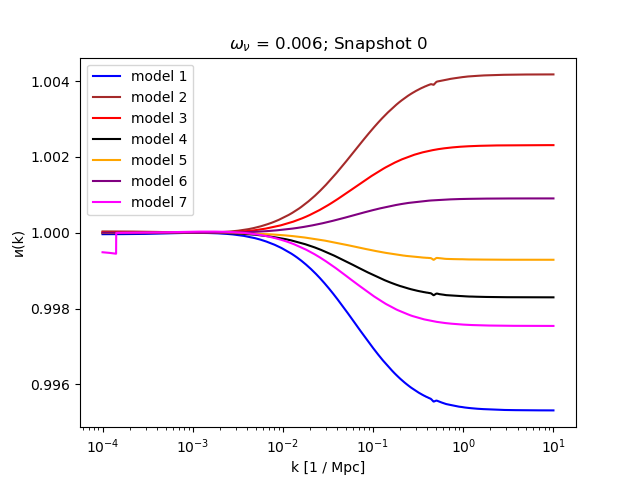
\includegraphics[width=\textwidth]{chap3/model_ratios}
 		\cprotect\caption{Example output of \verb|model_ratios|.}
 		\label{fig: model_ratios_demo}
    \end{subfigure}
    \begin{subfigure}{0.45 \textwidth}
    \centering
 		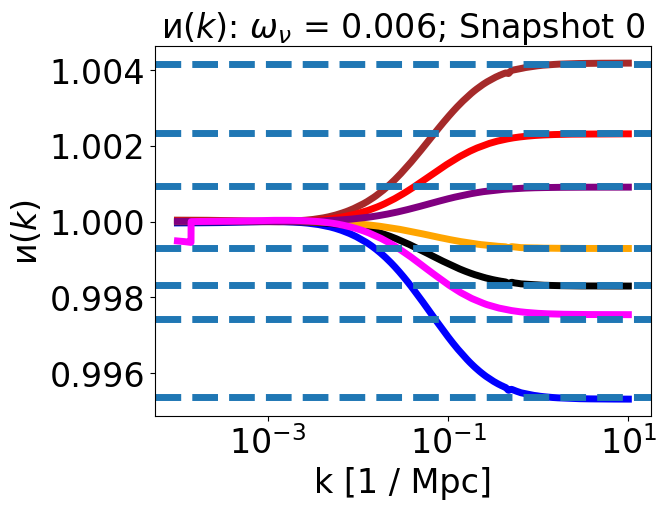
\includegraphics[width=\textwidth]{chap3/predictor_success}
 		\caption{With asymptote predictions.}
 		\label{fig: ee_prediction_demo}
    \end{subfigure}
        \centering
    \caption[$\ee$]
    		{Model ratios
    		\textcolor{red}{Would it have been better if I just included the
    		right plot and no left plot?}}
    \label{fig: model_ratios}
\end{figure}

\textcolor{orange}{The above paragraph only describes the function in the
case ``massive=`x'''}

\textcolor{green}{Both plot titles need to be redone.}

After experimenting with different functions and parameters, we find the
following fitting function:

\begin{equation}
\label{eq: fit}
\hat{\ee}_i = C \, \omega_\nu \, \ln \left( \frac{A_{s, i}}{A_{s, 0}} \right)
.\end{equation}

We demonstrate its predictions in figure~\ref{fig: ee_prediction_demo}.

We also show the errors for the Aletheia models in
figure~\ref{fit_errors_Aletheia}.

\section{Testing Functions}

To verify that our approach has general applicability, we now test the
asymptotic fit on a much broader selection of models.

\textcolor{orange}{What if we tested this fitting function on an independent
set of models with a consistent but different set of shape parameters?}

First, we created the function \verb|get_random_cosmology| function, which
accepts an $\omega_\nu$ value and returns a cosmology with randomized
evolution parameters over the following ranges:~\ref{tab: fit_test_params}.
All of the shape parameters are still consistent with Aletheia model 0.

\begin{table}[ht!]
\centering
\begin{tabular}{l|l|l}
\hline
Parameter & Minimum Value & Maximum Value \\ \hline
$\omega_\text{DE}$\footnotemark & 0.1 & 0.5 \\
$\omega_K$ & -0.05 & 0.05 \\
$w_0$ & -2.0 & -0.5 \\
$w_a$ & -0.5 & 0.5 \\
$A_s$\footnotemark & $5.003 \cdot 10^{-10}$ & $1.484 \cdot 10^{-8}$  \\
\end{tabular}
 \cprotect\caption[Parameter Ranges for Random Test
 	Cosmologies]{Parameters which we vary for the purpose of testing the
 	generality of fit~\ref{eq: fit}, and their domains.
 	\textcolor{red}{Is it poor form to have a footnote that looks like an
 	exponent? How should I do it differently?}}
 \label{tab: fit_test_params}
\end{table}

\addtocounter{footnote}{-1}

\footnotetext{Unfortunately, $\omega_\text{DE}$ is not accepted as an
input by CAMB's \verb|set_cosmology|. To vary $\omega_\text{DE}$ in this way,
we fix $\omega_b$ and $\omega_c$ and select a value for $\omega_K$. Then, we
vary $h$--according to equation~\ref{eq: h_to_omega}, this should only
affect $\omega_\text{DE}$.}

\footnotetext{These values were rounded to three significant figures. Refer
to the code for greater precision.}

These cosmologies cover a wide range of $\el$ values, as shown in
figure~\ref{fig: random_battery}. The errors for the fits are shown in
figure~\ref{fig: random_battery_errs}.

To further test our solution, we also created the function
\verb|get_As_matched_cosmology|, which randomizes the cosmologies in the same
way except for fixing $A_s$ at the value for model 0.
figure~\ref{fig: degenerate_battery}. The errors for the fits are shown in
figure~\ref{fig: degenerate_battery_errs}.

This third test demonstrates that the imperfections in our fit cannot be
attributed solely to the form of equation~\ref{eq: fit};  
since all of the cosmologies share $\omega_\nu$ and $A_s$ values, and since
the asymptotes were nevertheless not all identical, the
asymptote must have some dependence also on one of the other parameters that
we varied.  

However, the larger errors that we see in
figure~\ref{fig: random_battery_errs} suggests that our fit may only
approximately describe the relationship
between $A_s$, $\omega_\nu$, and the small-scale suppression of the power
spectrum. A symbolic regression investigation could prove highly effective at
resolving this ambiguity by efficiently searching out improved formulas. 
However, we do not consider this a promising avenue
for the continuation of this work (see section~\ref{sec: future_work} for our
recommendations); the error
is so low here that we do not believe the imperfect predictions to
significantly detract from the performance of the emulator.

\section{Summary of Findings}

% I'm not sure if this section will survive, we'll see how big the conclusion
% here ends up being.

In this chapter, we have illustrated how the scalar mode amplitude $A_s$
contains information of great relevance to the application of evolution
mapping to the emulation of massive-neutrino power spectra. As a result of 
these demonstrations, we know to construct 
our massive-neutrino emulator emulator over the six cosmological
parameters $\omega_b$, $\omega_c$, $n_s$, $\sigma_{12}$, $A_s$, and
$\omega_\nu$. In other words, to predict a power
spectrum, our emulator will accept as an input a vector describing
these six parameters. Conceptually, adding $A_s$ to the set of
emulation parameters allows us to treat $\omega_\nu$ like a shape
parameter.

Expansion of the parameter space represents the single most 
important novel step in this work. The remaining chapters will
focus on the integration of this modified evolution mapping framework
into a beginner-friendly emulation code.

\textcolor{blue}{Plot to do: add errors for original Aletheia set; add two
plots for random cosmology experiment; add two plots for fixed
A\_s experiment.}